
\chapter{Cinematica}
\minitoc
\section{\index{posizione}Vettore posizione}
\begin{Def}[vettore posizione]
  Fissato un sistema di riferimento cartesiano\footnote{per semplicità quasi sempre si parlerà del piano piuttosto che dello spazio, ma i risultati sono del tutto analoghi} $Oxy$ il vettore che congiunge l'origine con un punto $P$ è il \index{vettore!posizione}vettore posizione $\ve r$ che individua $P$ in quel sistema di riferimento.
\end{Def}
Poiché il punto può spostarsi nel tempo $\ve r$ sarà funzione del tempo $\ve r=\ve r(t)$ e descriverà al variare del tempo tutte le posizioni occupate da $P$ cioè la sua traiettoria\index{traiettoria}.

\begin{figure}[htbp]
  \centering
  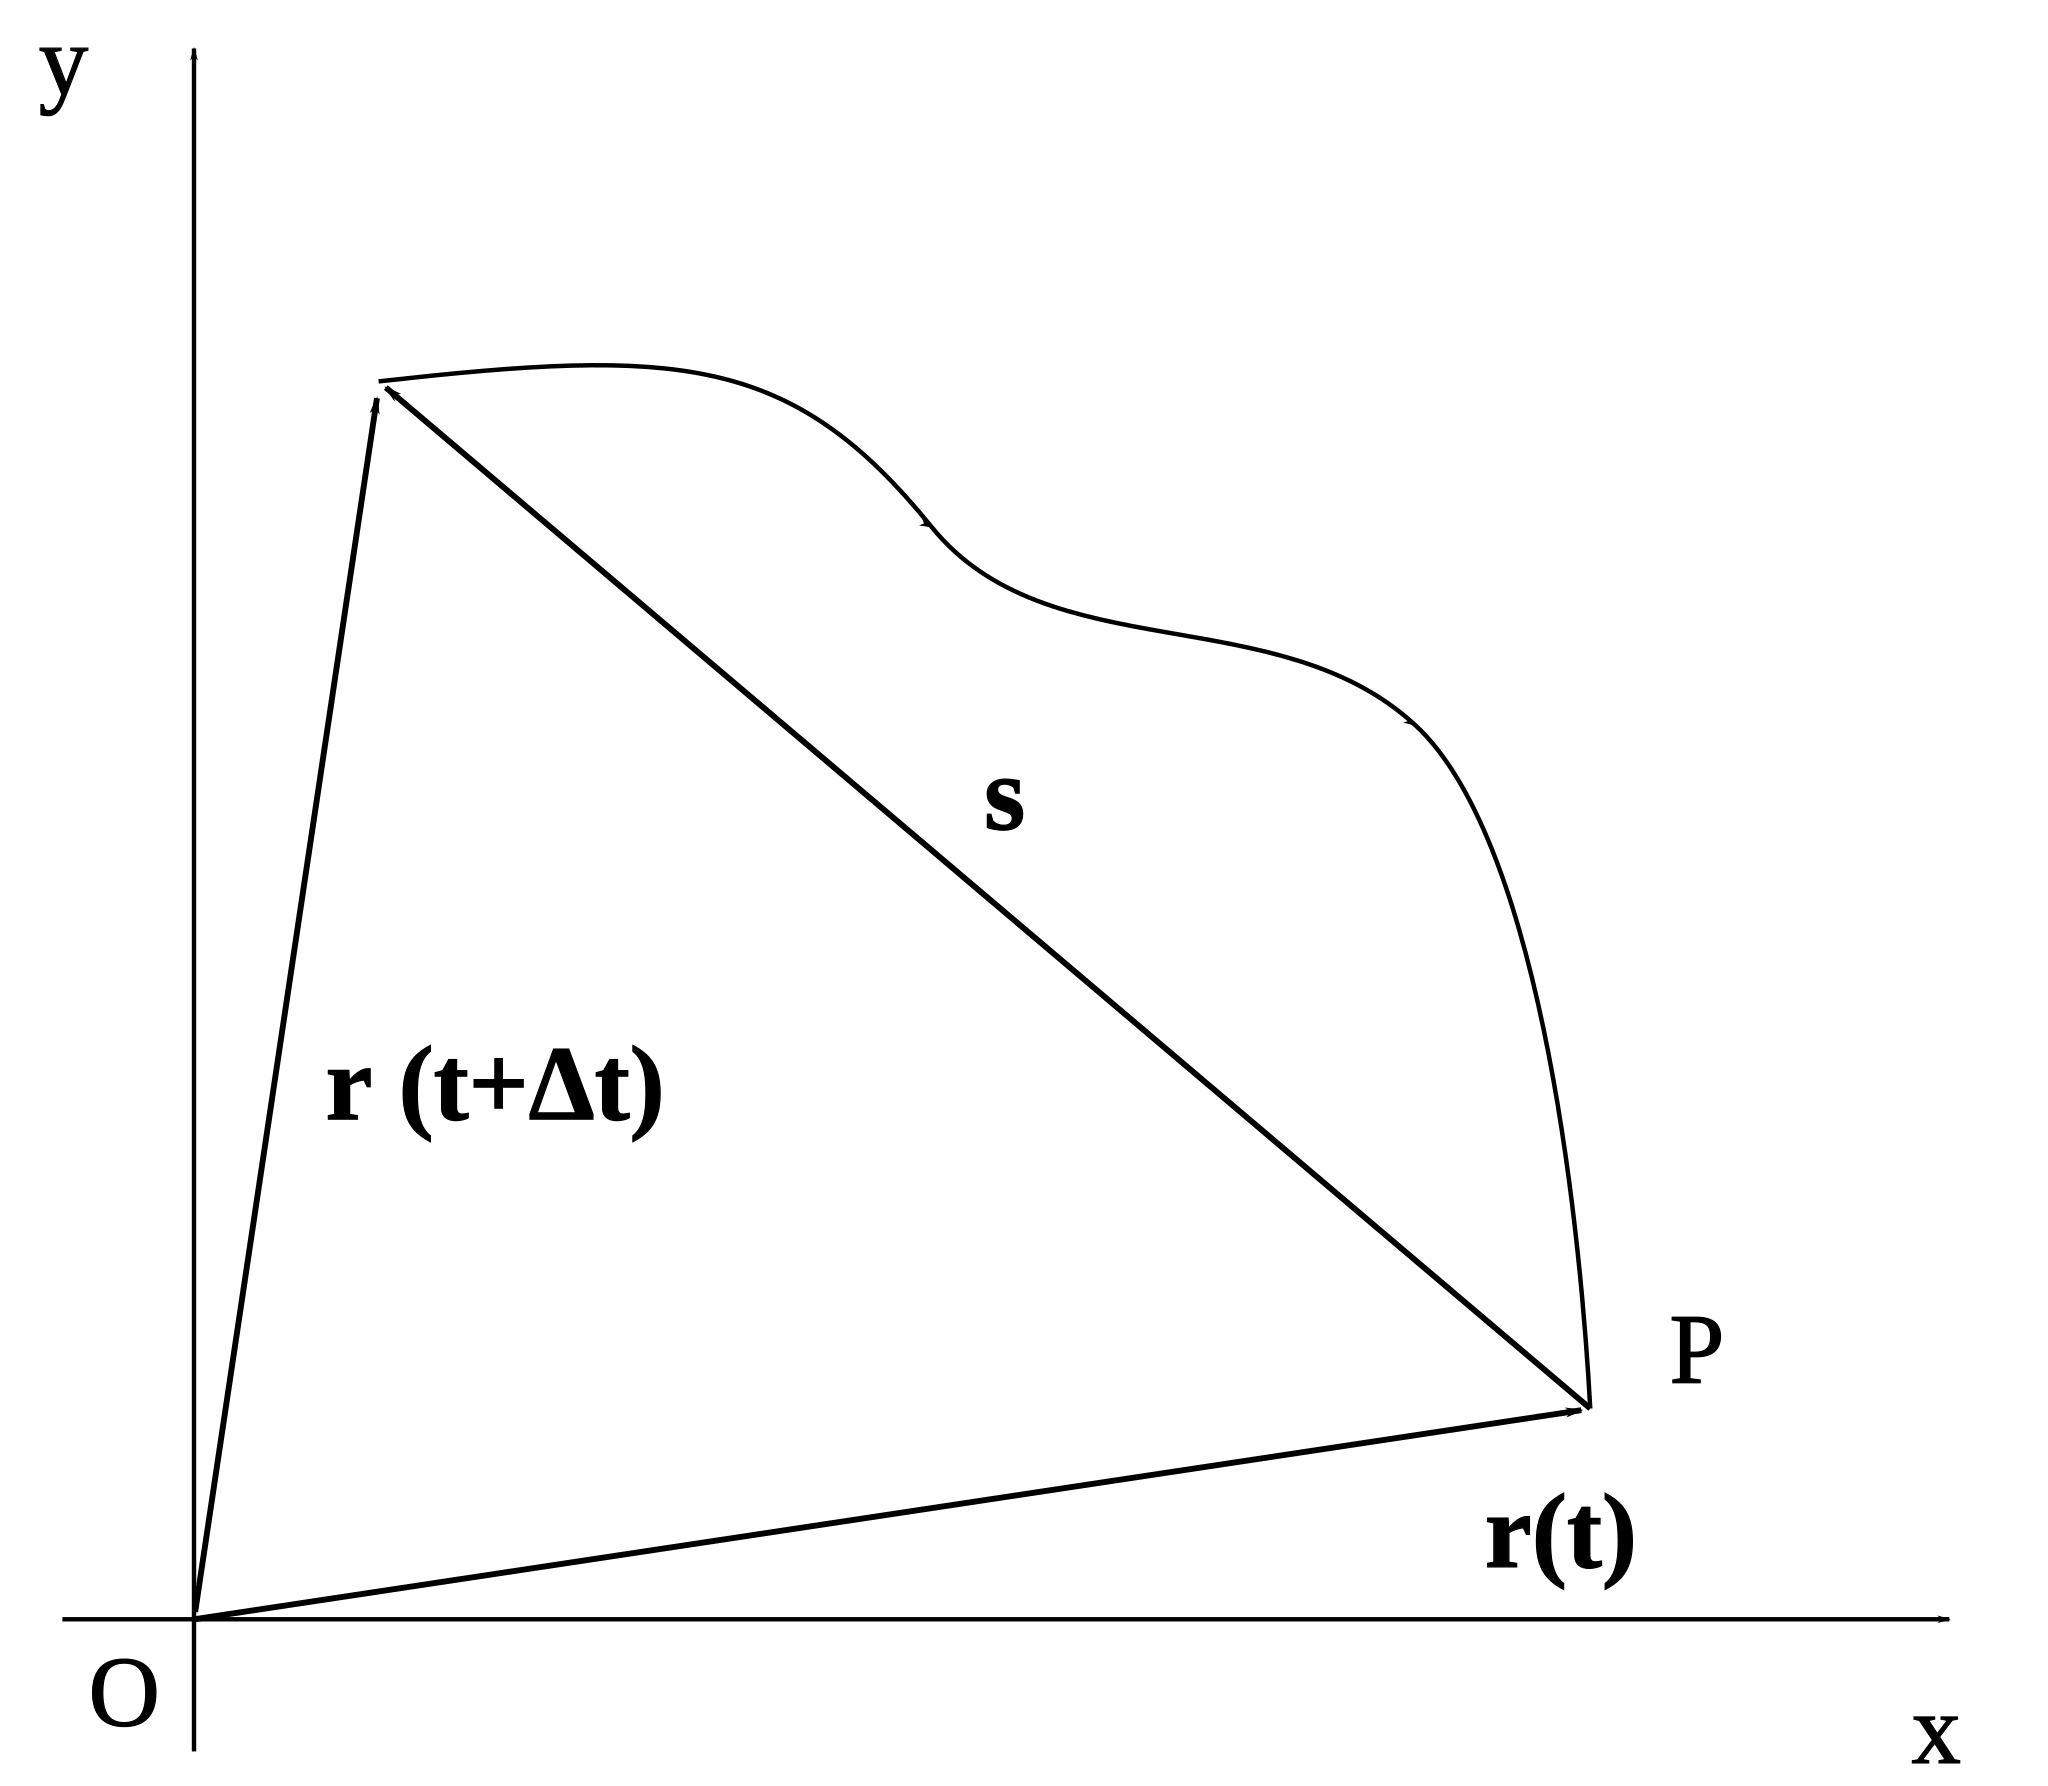
\includegraphics[scale=0.7]{immagini/fisica1/vettore_posizione}
  \caption{vettore posizione e spostamento.}
\end{figure}
\subsection{Vettore spostamento}
\begin{Def}[vettore spostamento]
  Il \index{vettore!spostemento} vettore spostamento è la variazione (differenza) del vettore posizione tra due istanti diversi:
  \begin{align*}
    \ve s\left(t,t+\Delta t\right) & =\Delta \ve r(t,t+\Delta t)                                                                                                                             \\
                                   & =\ve r\left(t+\Delta t\right)-\ve r\left(t\right)=x\left(t+\Delta t\right)\ve i+y\left(t+\Delta t\right)\ve j-x\left(t\right)\ve i-y\left(t\right)\ve j \\
                                   & =\left[x(t+\Delta t)-x(\Delta t)\right]\ve i+[y(t+\Delta t)-y(t)]\ve j=\Delta x\ve i+\Delta y \ve j
  \end{align*}
\end{Def}
\section{\index{velocità}Vettore velocità}
\begin{Def}[\index{velocità!media}Velocità Media]
  \[\ve v_m(t,t+\Delta t)=\frac{\Delta\ve r(t,t+\Delta t)}{\Delta
      t}=\frac{1}{\Delta t}\{\Delta x\ve i+\Delta y\ve
    j\}=\frac{\Delta x}{\Delta t}\ve i+\frac{\Delta y}{\Delta t}\ve
    j\]
\end{Def}
\begin{Def}[\index{velocità!istantanea}Velocità Istantanea]
  \[\ve v(t)=\lim_{\Delta t\rightarrow 0}\ve v_m(t,t+\Delta t)=\lim_{\Delta t\rightarrow 0} \frac{\Delta\ve r}{\Delta t}(t)={\left.\frac{\ud \ve r}{\ud t}\right|_t}=\left.\frac{\ud x}{\ud t}\right|_t\ve i+\left.\frac{\ud y}{\ud t}\right|_t\ve j\]
\end{Def}
Si noti che la norma della derivata non è la derivata della norma:
\[\norm{\ve v}=\norm{\frac{\ud\ve r}{\ud t}}\neq\frac{\ud}{\ud t}\norm{\ve r}\]
\begin{Def}[\index{velocità!scalare}Velocità Scalare]
  \[v_s=\frac{\text{spazio totale percorso}}{\Delta t}\]
\end{Def}
\section{\index{accelerazione}Vettore accelerazione}
\begin{Def}[accelerazione istantanea]
  \[\ve a=\frac{\ud \ve v}{\ud t}={\frac{\ud^2 \ve r}{\ud t^2}}\]
\end{Def}
\section[Moto rettilineo uniforme]{\index{moto!rettilineo uniforme}Moto rettilineo uniforme\protect\footnote{usiamo sempre condizioni iniziali implicite, del tipo $t_0=0$, $\ve r(0)=\ve r_0$, $\ve v(0)=\ve v_0$}}
\begin{Def}[moto rettilineo uniforme]
  \[\ve v=\overrightarrow\const\]
\end{Def}
\[\ud\ve r=\ve v\,\ud t\qquad\int_{\ve r_0}^{\ve r}\ud\ve r=\int_0^t\ve v\,\ud t \qquad \ve r-\ve r_0=\ve v t\]
\begin{eqimp}{equation}
  \ve r=\ve v t+\ve r_0
\end{eqimp}
\section{\index{moto!uniformemente accelerato}Moto uniformemente accelerato}
\begin{Def}[moto uniformemente accelerato]
  \[\ve a=\overrightarrow{\const}\]
\end{Def}
\[\ve a\,\ud t=\ud \ve v\qquad\int_0^t\ve a\,\ud t=\int_{\ve v_0}^{\ve v}\ud \ve v\qquad\ve a t=\ve v-\ve v_0\]
\begin{eqimp}{equation}
  \ve v=\ve a t+\ve v_0
  \label{vt_01}
\end{eqimp}
\[\ve v=\ve a t+\ve v_0=\frac{\ud \ve r}{\ud t}\]
\[\ud \ve r=\left(\ve a t+\ve v_0\right)\ud t\qquad\int_{\ve r_0}^{\ve r}\ud \ve r=\int_0^t\left(\ve a t+\ve v_0\right)\ud t\qquad\ve r-\ve r_0=\frac{1}{2}\ve a t^2+\ve v_0 t\]
\begin{eqimp}{equation}
  \ve r=\frac{1}{2}\ve a t^2+\ve v_0 t+\ve r_0
  \label{vt_02}
\end{eqimp}
\subsection{Velocità in funzione dello spazio}
In certi casi può risultare molto comoda la formula relativa al
moto uniformemente accelerato scritta in questo modo:
\begin{equation}
  v^2-v_0^2=2a(r-r_0)
  \label{vt_03}
\end{equation}
che vale solo nel caso unidimensionale\footnote{nel caso unidimensionale le \eqref{vt_01} e la \eqref{vt_02} si scrivono come:
  \begin{equation}
    v(t)=at+v_0\qquad r(t)=\frac{1}{2}at^2+v_0t+r_0
  \end{equation}
  eliminiamo il tempo per trovare $v(r)$: ricaviamo $t$ dalla prima e sostituiamolo nella seconda, semplifichiamo e otteniamo la \eqref{vt_03}}.
\section{\index{moto!circolare!uniforme}Moto circolare uniforme}
Per moto circolare uniforme si intende quel moto su traiettoria
circolare di raggio $R$ in cui il modulo del vettore velocità rimane costante
nel tempo (mentre la sua direzione varia ed è sempre tangente
alla circonferenza). Definiamo la velocità angolare\index{velocità!angolare}\index{omega@$\omega$|see{velocità angolare}}: $\omega=\frac{\ud\theta}{\ud t}$ e l'accelerazione angolare\index{accelerazione!angolare}\index{alpha@$\alpha$|see{accelerazione angolare}} $\alpha=\frac{\ud \omega}{\ud t}$; in realtà possono essere definiti come vettori.
\[\norm{\ve v}=\const\]
\[\text{scegliamo $\ve r(t=0)=\ve r_0$}:\left\{
  \begin{array}{l}
    x=R \\
    y=0 \\
  \end{array}\right.\]
\[\ve r=R\cos\theta\ve i+R\sin\theta\ve j\]
\[\theta=\frac{\text{arco}}{\text{raggio}}=\frac{vt}{R}=\omega t\qquad\omega=\dot\theta=\frac{v}{R}=\const\]
\[\ve r=R\cos(\omega t)\ve i+R\sin(\omega t)\ve j\]
\[\ve v=\frac{\ud \ve r}{\ud t}=-R\omega\sin(\omega t)\ve
  i+R\omega\cos(\omega t)\ve j\]
\begin{align*}|\ve v|^2 & =v_x^2+v_y^2=R^2\omega^2\sin^2(\omega
              t)+R^2\omega^2\cos^2(\omega t)                                               \\
                        & =R^2\omega^2\left(\sin^2\left(\omega t\right)+\cos^2\left(\omega
              t\right)\right)=R^2\omega^2
\end{align*}
\[v=\omega R\]
\[\ve v\cdot\ve r=0\Rightarrow\ve v\bot\ve r\]
\[\ve v\cdot\ve r=v_xx+v_yy=-R\omega\sin(\omega t)R\cos(\omega t)+R\omega\cos(\omega t)R\sin(\omega t)=0\]
\begin{align*}
  \ve a & =\frac{\ud\ve v}{\ud t}=-R\omega^2\cos(\omega t)\ve
  i-R\omega^2\sin(\omega t)\ve j                              \\
        & =-R\omega^2\left(\cos\left(\omega t\right)\ve i+
  \sin\left(\omega t\right)\ve j\right)=-\omega^2\ve r
\end{align*}
\[|\ve a|^2=R^2\omega^4\cos^2(\omega t)+R^2\omega^4\sin^2(\omega
  t)=R^2\omega^4\]
\[a=\omega^2R=\omega v=\frac{v^2}{R}\]
\section{\index{moto!circolare}Moto circolare}
\begin{figure}[htbp]
  \centering
  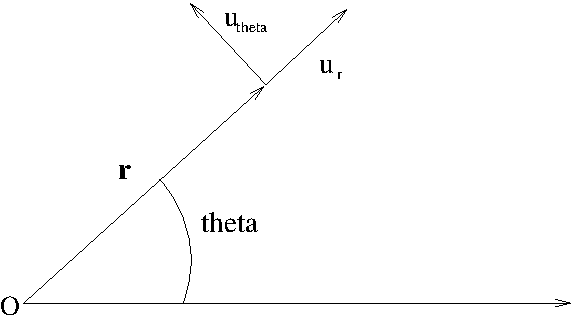
\includegraphics[scale=1]{immagini/fisica1/CorPol}
  \caption{\index{coordinate!polari}Coordinate polari.}
\end{figure}
\[\ve r=R\ve u_r\]
\[
  \left\{\begin{array}{ll}
    \ve u_r=\cos\theta(t)\ve i+\sin\theta(t)\ve j \\
    \ve u_\theta=-\sin\theta(t)\ve i+\cos\theta(t)\ve j
  \end{array}\right.
\]
\[\frac{\ud\ve u_\theta}{\ud t}=-\dot{\theta}\cos\theta\ve i-\dot{\theta}\sin\theta\ve j=-\dot{\theta}\ve u_r\]
\begin{align*}
  \ve v & =\frac{\ud \ve r}{\ud t}=\frac{\ud\left(R\ve
    u_r\right)}{\ud t}=R\frac{\ud \ve u_r}{\ud
  t}                                                                 \\
        & =R\left(-\dot\theta\sin\theta\ve i+\dot\theta\cos\theta\ve
  j\right)=R\dot\theta\ve u_\theta
\end{align*}
\[\ve a=\frac{\ud\ve v}{\ud t}=\frac{\ud\left(R\dot\theta\ve
    u_\theta\right)}{\ud t}=R\ddot\theta\ve
  u_\theta+R\dot\theta\frac{\ud\ve u_\theta}{\ud
    t}=R\ddot\theta\ve u_\theta-R\dot\theta^2\ve u_r\]


\section{\index{moto!in coordinate polari}Moto qualsiasi in coordinate polari}
\[\ve r(t)=r\ve u_r\]
\[\ve u_r=\cos\theta\ve i+\sin\theta\ve j\qquad \ve u_\theta=-\sin\theta\ve i+\cos\theta\ve j\]
\[\frac{\ud\ve u_r}{\ud t}=-\dot\theta\sin\theta\ve
  i+\dot\theta\cos\theta\ve j=\dot\theta\left(-\sin\theta\ve
  i+\cos\theta\ve j\right)=\dot\theta\ve u_\theta\]
\[\frac{\ud\ve u_\theta}{\ud t}=-\dot\theta\cos\theta\ve
  i-\dot\theta\cos\theta\ve j=-\dot\theta\left(\cos\theta\ve
  i+\sin\theta\ve j\right)=-\dot\theta\ve u_r\]
\[\ve v=\frac{\ud\ve r}{\ud t}=\dot r\ve u_r+r\frac{\ud\ve
    u_r}{\ud t}=\dot r\ve u_r+r\dot\theta\ve u_\theta\]
\[\ve a=\frac{\ud\ve v}{\ud t}=\ddot r\ve u_r+\dot
  r\dot\theta\ve u_\theta+\dot r\dot\theta\ve
  u_\theta+r\ddot\theta\ve u_\theta-r\dot\theta^2\ve u_r=\ve
  u_r\left(\ddot r-r\dot\theta^2\right)+\ve u_\theta\left(2\dot
  r\dot\theta+r\ddot\theta\right)\]

I vettori velocità e accelerazione vengono scomposti in due
componenti:
\begin{enumerate}
  \item[--] \index{velocità!radiale}Velocità radiale: $v_r=\dot r$
  \item[--] \index{velocità!perpendicolare}Velocità perpendicolare: $v_\theta=r\dot\theta$
  \item[--] \index{accelerazione!radiale}Accelerazione radiale: $a_r=\ddot r-r\dot\theta^2$
  \item[--] \index{accelerazione!perpendicolare}Accelerazione perpendicolare: $a_\theta=2\dot r\dot\theta+r\ddot
      \theta$
\end{enumerate}
\section{\index{moto!armonico}Moto armonico}
\begin{figure}[htbp]
  \centering
  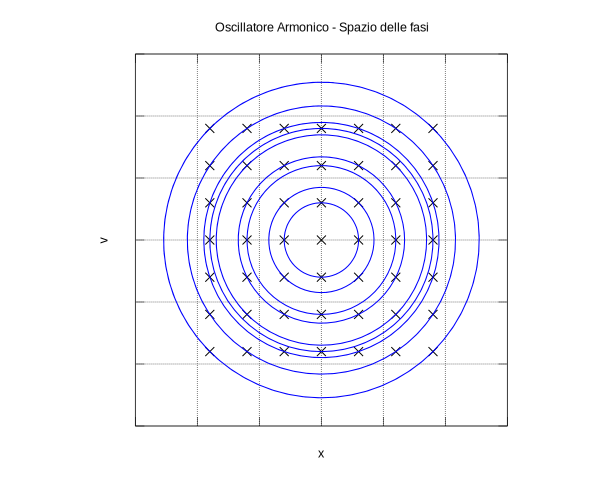
\includegraphics[scale=0.6]{immagini/fisica1/oscillatore_fase}
  % oscillatore_fase.: 480x384 pixel, 72dpi, 16.93x13.55 cm, bb=0 0 480 384
  \caption{Traiettorie nello spazio delle configurazioni dell'oscillatore armonico a partire da diverse condizioni iniziali.}
\end{figure}
Il moto armonico è un moto con equazione differenziale:
\begin{eqimp}{equation}
  \ddot x=-\omega^2 x
\end{eqimp}
la cui soluzione è:
\[x=A\sin(\omega t+\varphi)\]
derivando si ottiene
\[v=\frac{\ud x}{\ud t}=A\omega\cos(\omega t+\varphi)\]
\[a=\frac{\ud v}{\ud t}=-A\omega^2\sin(\omega t+\varphi)\]
ovviamente risulta che: $a = -\omega^2 x=\ddot x$.
Per esempi (pendoli, molle) vedi sezione \ref{armonico} a pagina \pageref{armonico}.
\subsection{Moto armonico smorzato\index{moto!armonico!smorzato}}
\begin{figure}
  \centering
  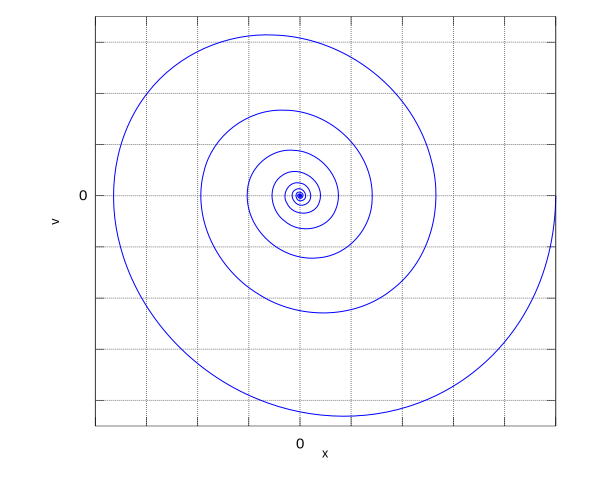
\includegraphics[scale=0.6]{immagini/fisica1/oscillatore_smorzato_fase}
  % oscillatore_smorzato_fase.pdf: 480x384 pixel, 72dpi, 16.93x13.55 cm, bb=0 0 480 384
  \caption{Traiettorie nello spazio delle configurazioni dell'oscillazione smorzato con coefficiente di attrito debole.}
\end{figure}
Introduciamo nel moto armonico una forza smorzatrice, per esempio una forza d'attrito che varia con la velocità:
\[F=-\gamma \frac{\ud x}{\ud t}\]
\[m\ddot x=-kx-\gamma\dot x\qquad m\ddot x+\gamma\dot x+kx=0\]
$\tau=\frac{m}{\gamma}$ è un tempo, la frequenza del moto armonico non smorzato è $\frac{k}{m}=\omega_0^2$
\[\ddot x+\frac{\gamma}{m}\dot x+\frac{k}{m}x=0\qquad \ddot x+\frac{1}{\tau}\dot x+\omega_0^2x=0\]
se $\tau=\infty$ allora il moto non è più smorzato.

Una soluzione è:
\[x(t)=e^{st}\]
\[\dot x(t)=sx(t)\qquad \ddot x(t)=s^2x(t)\]
\[s^2x(t)+\frac{1}{\tau}sx(t)+\omega_0^2x(t)=0\]
\[s_{1/2}=\dfrac{-\dfrac{1}{\tau}\pm\sqrt{\dfrac{1}{\tau^2}-4\omega_0^2}}{2}=-\frac{1}{2\tau}\pm\sqrt{\frac{1}{4\tau^2}-\omega_0^2}\]
quindi la soluzione generale è una combinazione lineare delle soluzioni:
\[
  x(t)=A_1e^{s_1t}+A_2e^{s_2t}
\]
a seconda che le radici del polinomio siano reali o complesse si possono distinguere due casi:
\begin{description}
  \item[attrito forte]
    \[\beta=\frac{1}{4\tau^2}-\omega_0^2>0\qquad\tau<\frac{1}{2\omega_0}\qquad\gamma>2\sqrt{km}\]
    \[s_{1/2}=-\frac{1}{2\tau}\pm\beta\qquad\text{radici reali e}<0\]
    \[x(t)=A_1e^{s_1t}+A_2e^{s_2t}\]
  \item[attrito debole]
    \[\frac{1}{4\tau^2}-\omega_0^2<0\qquad \tau>\frac{1}{2\omega_0}\qquad\gamma<2\sqrt{km}\]
    \[s_{1/2}=\dfrac{-\dfrac{1}{\tau}\pm\sqrt{\dfrac{1}{\tau^2}-4\omega_0^2}}{2}=-\frac{1}{2\tau}\pm i\omega\]
    \begin{align*}x(t) & =A_1e^{s_1it}+A_2e^{s_2it}=A_1e^{-\frac{t}{2\tau}-i\omega t}+A_2e^{-\frac{t}{2\tau}+i\omega t}=                    \\
                   & =e^{-\frac{t}{2\tau}}\left(A_1e^{-i\omega t}+A_2e^{i\omega t}\right)=A e^{-\frac{t}{2\tau}}\sin(\omega t +\varphi)\end{align*}
    quindi è un moto armonico con frequenza $\omega=\sqrt{\omega_0-\frac{1}{4\tau^2}}$ la cui ampiezza diminuisce con un fattore frenante $e^{-\frac{t}{2\tau}}$.\footnote{Il caso critico in cui ci siano due radici coincidenti è tralasciato poiché puntiforme}
\end{description}

\section{\index{trasformazioni!di Galileo}Trasformazioni di Galileo}
Le trasformazioni di Galileo sono equazioni valide nella meccanica classica che consentono di descrivere le coordinate di un sistema rispetto alle di coordinate di un altro sistema che si muove di moto rettilineo uniforme rispetto al primo. Un sistema è detto inerziale se vale la prima legge di Newton. Se in un sistema è inerziale allora un altro sistema è inerziale se e solo se si muove di motto rettilineo uniforme rispetto al primo.
\newline

Primo osservatore ``fermo'':$\qquad O\quad\ve r\quad\;\ve
  v\quad\;\ve a$

Secondo osservatore in moto:$\quad O'\quad\!\ve r\,'\quad\!\ve
  v\,'\quad\!\ve a\,'$

In meccanica classica si assume:$\quad t=t'$

$\ve u$ velocità di trascinamento: \index{velocità!relativa}velocità di $O'$ rispetto ad $O$.
\begin{legge}
  $\ve r(t)=\overrightarrow{\left(O'-O\right)}+\ve r\,'=\ve u
    t+\ve r\,'$
\end{legge}
\begin{legge}[composizione delle velocità]
  \index{composizione delle velocità}
  \[\ve v=\frac{\ud\ve r}{\ud t}=\frac{\ud}{\ud t}\left(\ve u
    t+\ve r\,'\right)=\frac{d}{\ud t}\left(\ve u
    t\right)+\frac{\ud\ve r\,'}{\ud t}=\ve u+\frac{\ud\ve r\,'}{\ud
      t'}=\ve u+\ve v\,'\]
  velocità assoluta = velocità relativa + \index{velocità!di trascinamento}velocità di trascinamento
\end{legge}
\begin{legge}[invarianza dell'accelerazione]
  \[\ve a=\frac{\ud \ve v}{\ud t}=\frac{\ud}{\ud t}(\ve u+\ve
    v\,')=0+\frac{\ud \ve v\,'}{\ud t}=\frac{\ud \ve v\,'}{\ud
      t'}=\ve a'\]
  L'accelerazione quindi è invariante
\end{legge}
\[\left\{\begin{array}{ll}
    \ve r=\ve r\,'+\ve u t & \text{trasformate di Galileo}        \\
    \ve v=\ve u+\ve v\,'   & \text{somma delle velocità}          \\
    \ve a=\ve a\,'         & \text{invarianza dell'accelerazione} \\
    t=t'                   & \text{ipotesi del tempo assoluto}    \\
  \end{array}\right.\]
Esse valgono nell'ipotesi che se $t=0=t'$ allora $\ve r\,'=\ve r$.
Non esiste un sistema di riferimento assoluto.
\begin{Es}[lancio del sasso]
  Consideriamo due sistemi inerziali $O$ e $O'$. $O$ veda $O'$ muoversi lungo l'asse $x$ con velocità $\ve w$. Siano gli assi $y$ e $z$ uguali nei due sistemi. $O$ lancia un sasso verso l'alto, le equazioni del moto per il sasso visto da $O$ sono:
  \begin{gather*}
    x(t) = x_0\\
    y(t) = -\frac{1}{2}gt^2 + v_0 t
  \end{gather*}
  la traiettoria in questo caso è un segmento verticale con gli estremi in $(x_0,0)$ e $(x_0,\frac{v_0^2}{2g})$. Nel sistema $O'$ invece questo moto diventa:
  \begin{gather*}
    x'(t) = x(t) - w t = x_0 - wt\\
    y(t) = -\frac{1}{2}gt^2 + v_0 t
  \end{gather*}
  si noti che $v_0$ è sempre lo stesso nei due sistemi. Eliminando il tempo: $t = (x_0-x') /w$ si ottiene l'equazione di una parabola il cui vertice è ad una altezza uguale a quella nel sistema di $O$.
\end{Es}

\subsection{Invarianza e covarianza\index{invarianza}\index{covarianza}}
Una grandezza si dice invariante se è numericamente uguale alla sua trasformata, cioè $x=T(x)=x'$. Nelle trasformazioni di Galileo l'accelerazione è invariante rispetto alla trasformazione che trasforma le coordinate di $O$ in quelle di $O'$. Nella relatività galileiana la lunghezza è invariante, nella relatività ristretta no.

Una legge si dice covariante se la sua espressione è uguale alla sua trasformata, cioè $f(x)=T(f(x))$.